\section{Results}


\subsection{Number of iterations}

\begin{figure}[H]
  \centering
  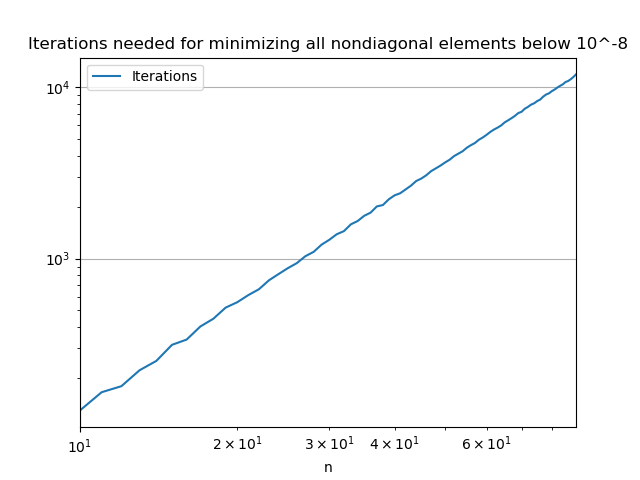
\includegraphics[width=0.66\textwidth]{../figures/iterations.png}

  \caption{Runs of the Jacobi method implemented in c++. Number of iterations
  needed to make all offdiagonal elements smaller than 10$^{-8}$ as function of
  matrix size n.}

  \label{fig:iterations}
\end{figure}

\subsection{Timing Result}

\begin{figure}[H]
  \centering
  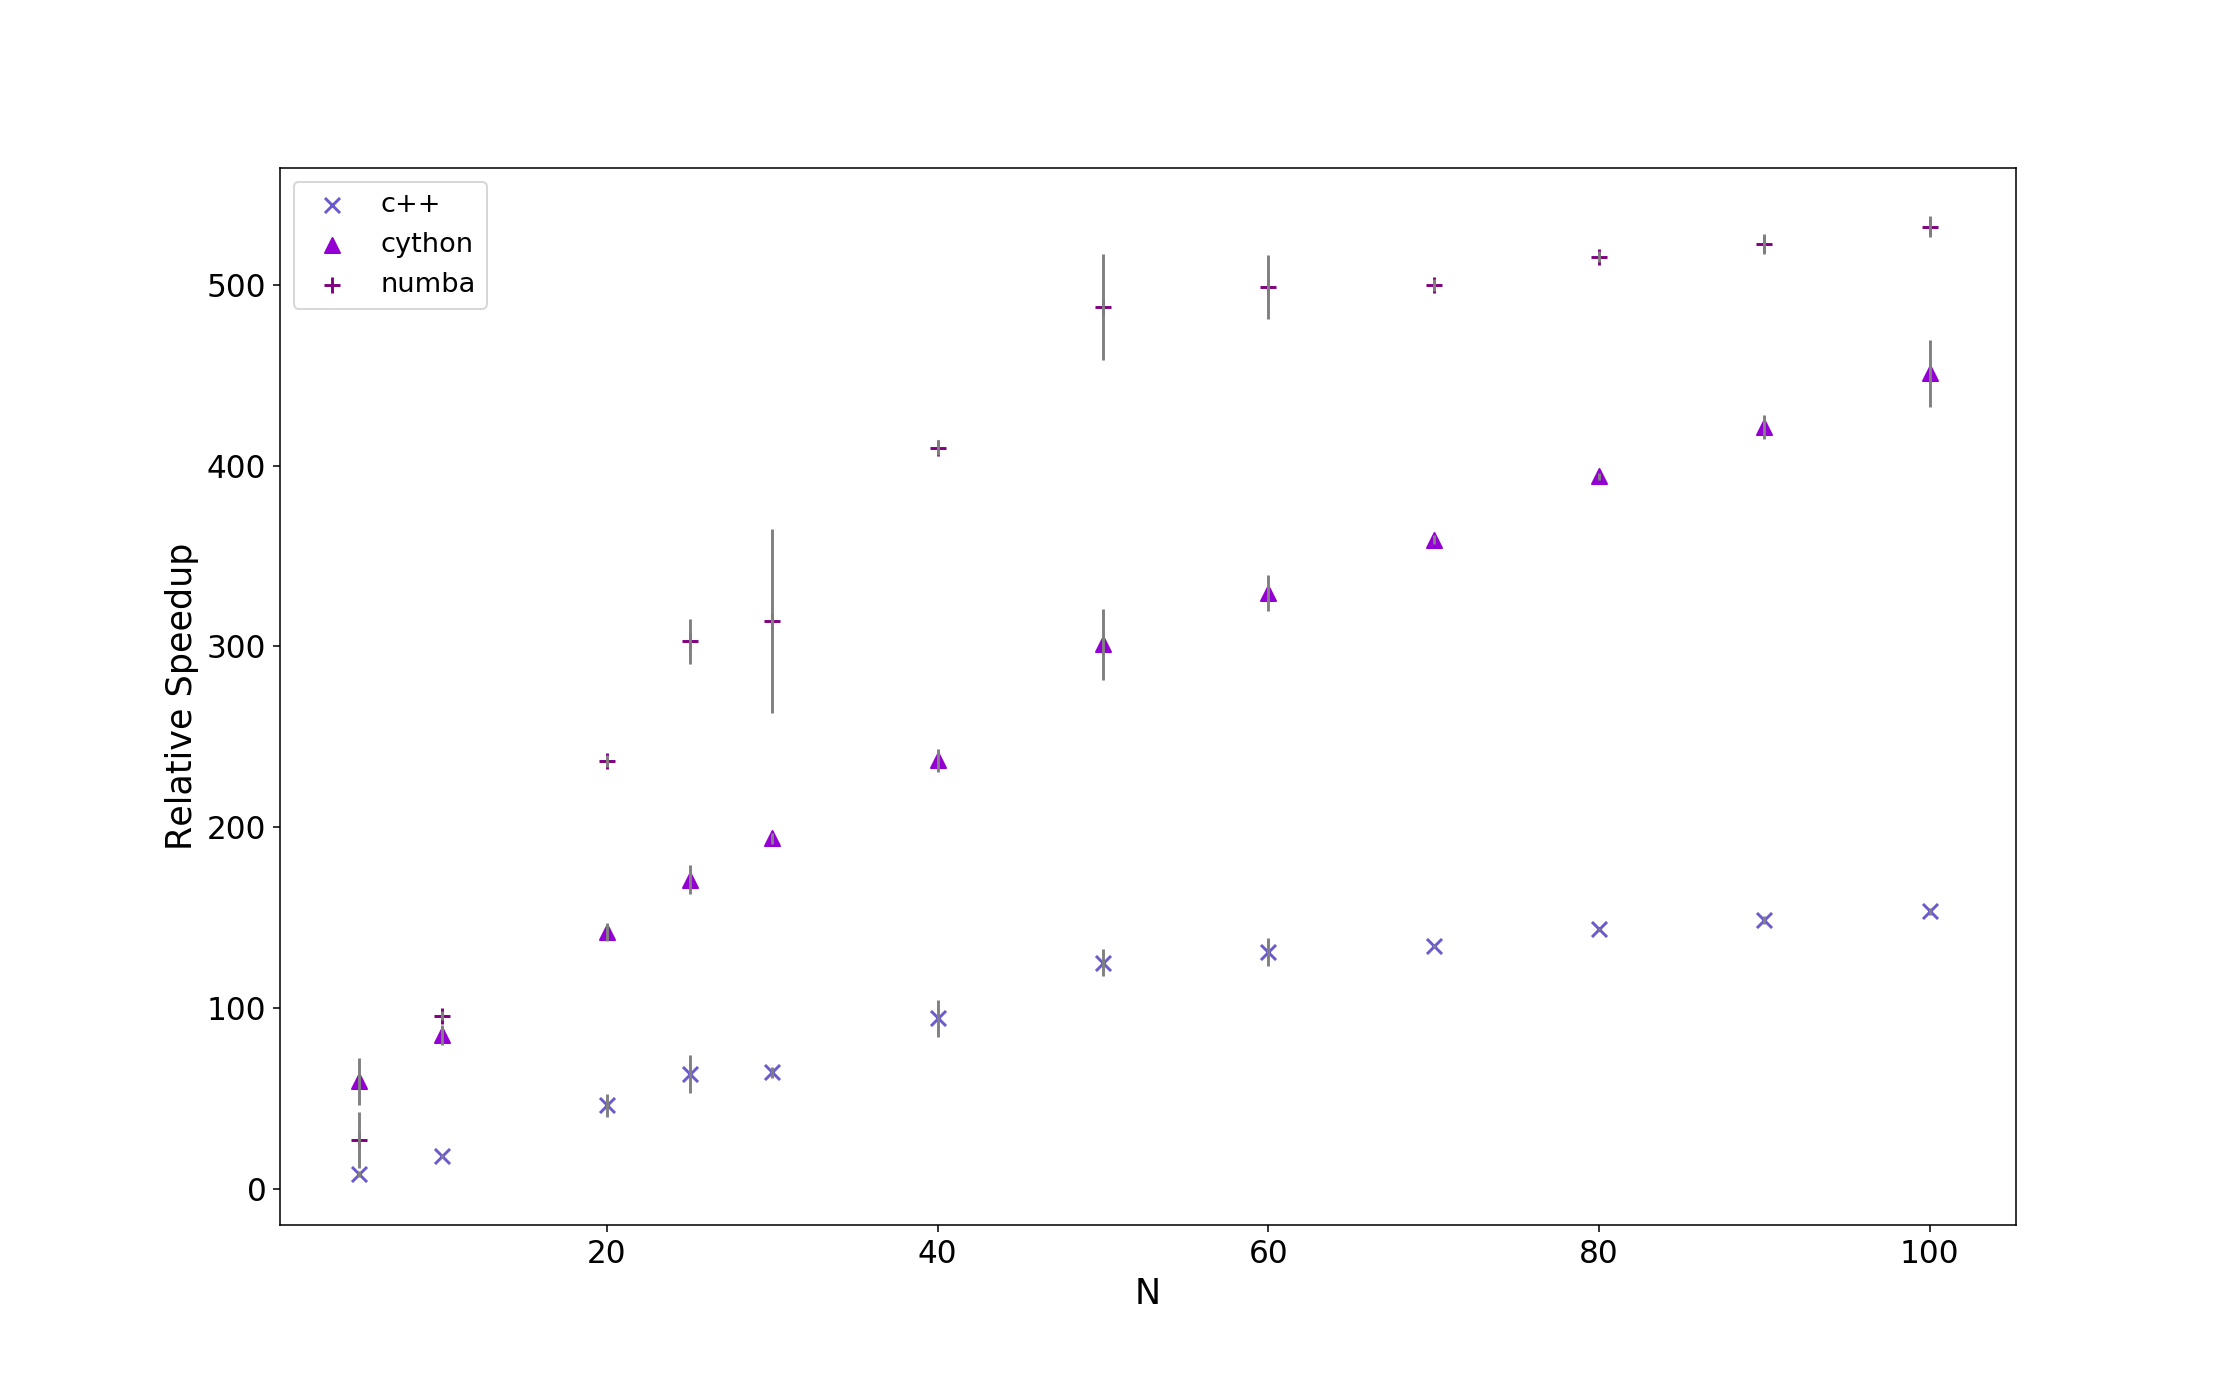
\includegraphics[width=1.0\textwidth]{../figures/avgspeed.png}
  \caption{ The average timing of 5 runs, divided by the average of the standard
  python timings. Starting from $N=5$ until $N=100$. }
  \label{fig:comp_python}
\end{figure}

\begin{figure}[H]
  \centering
  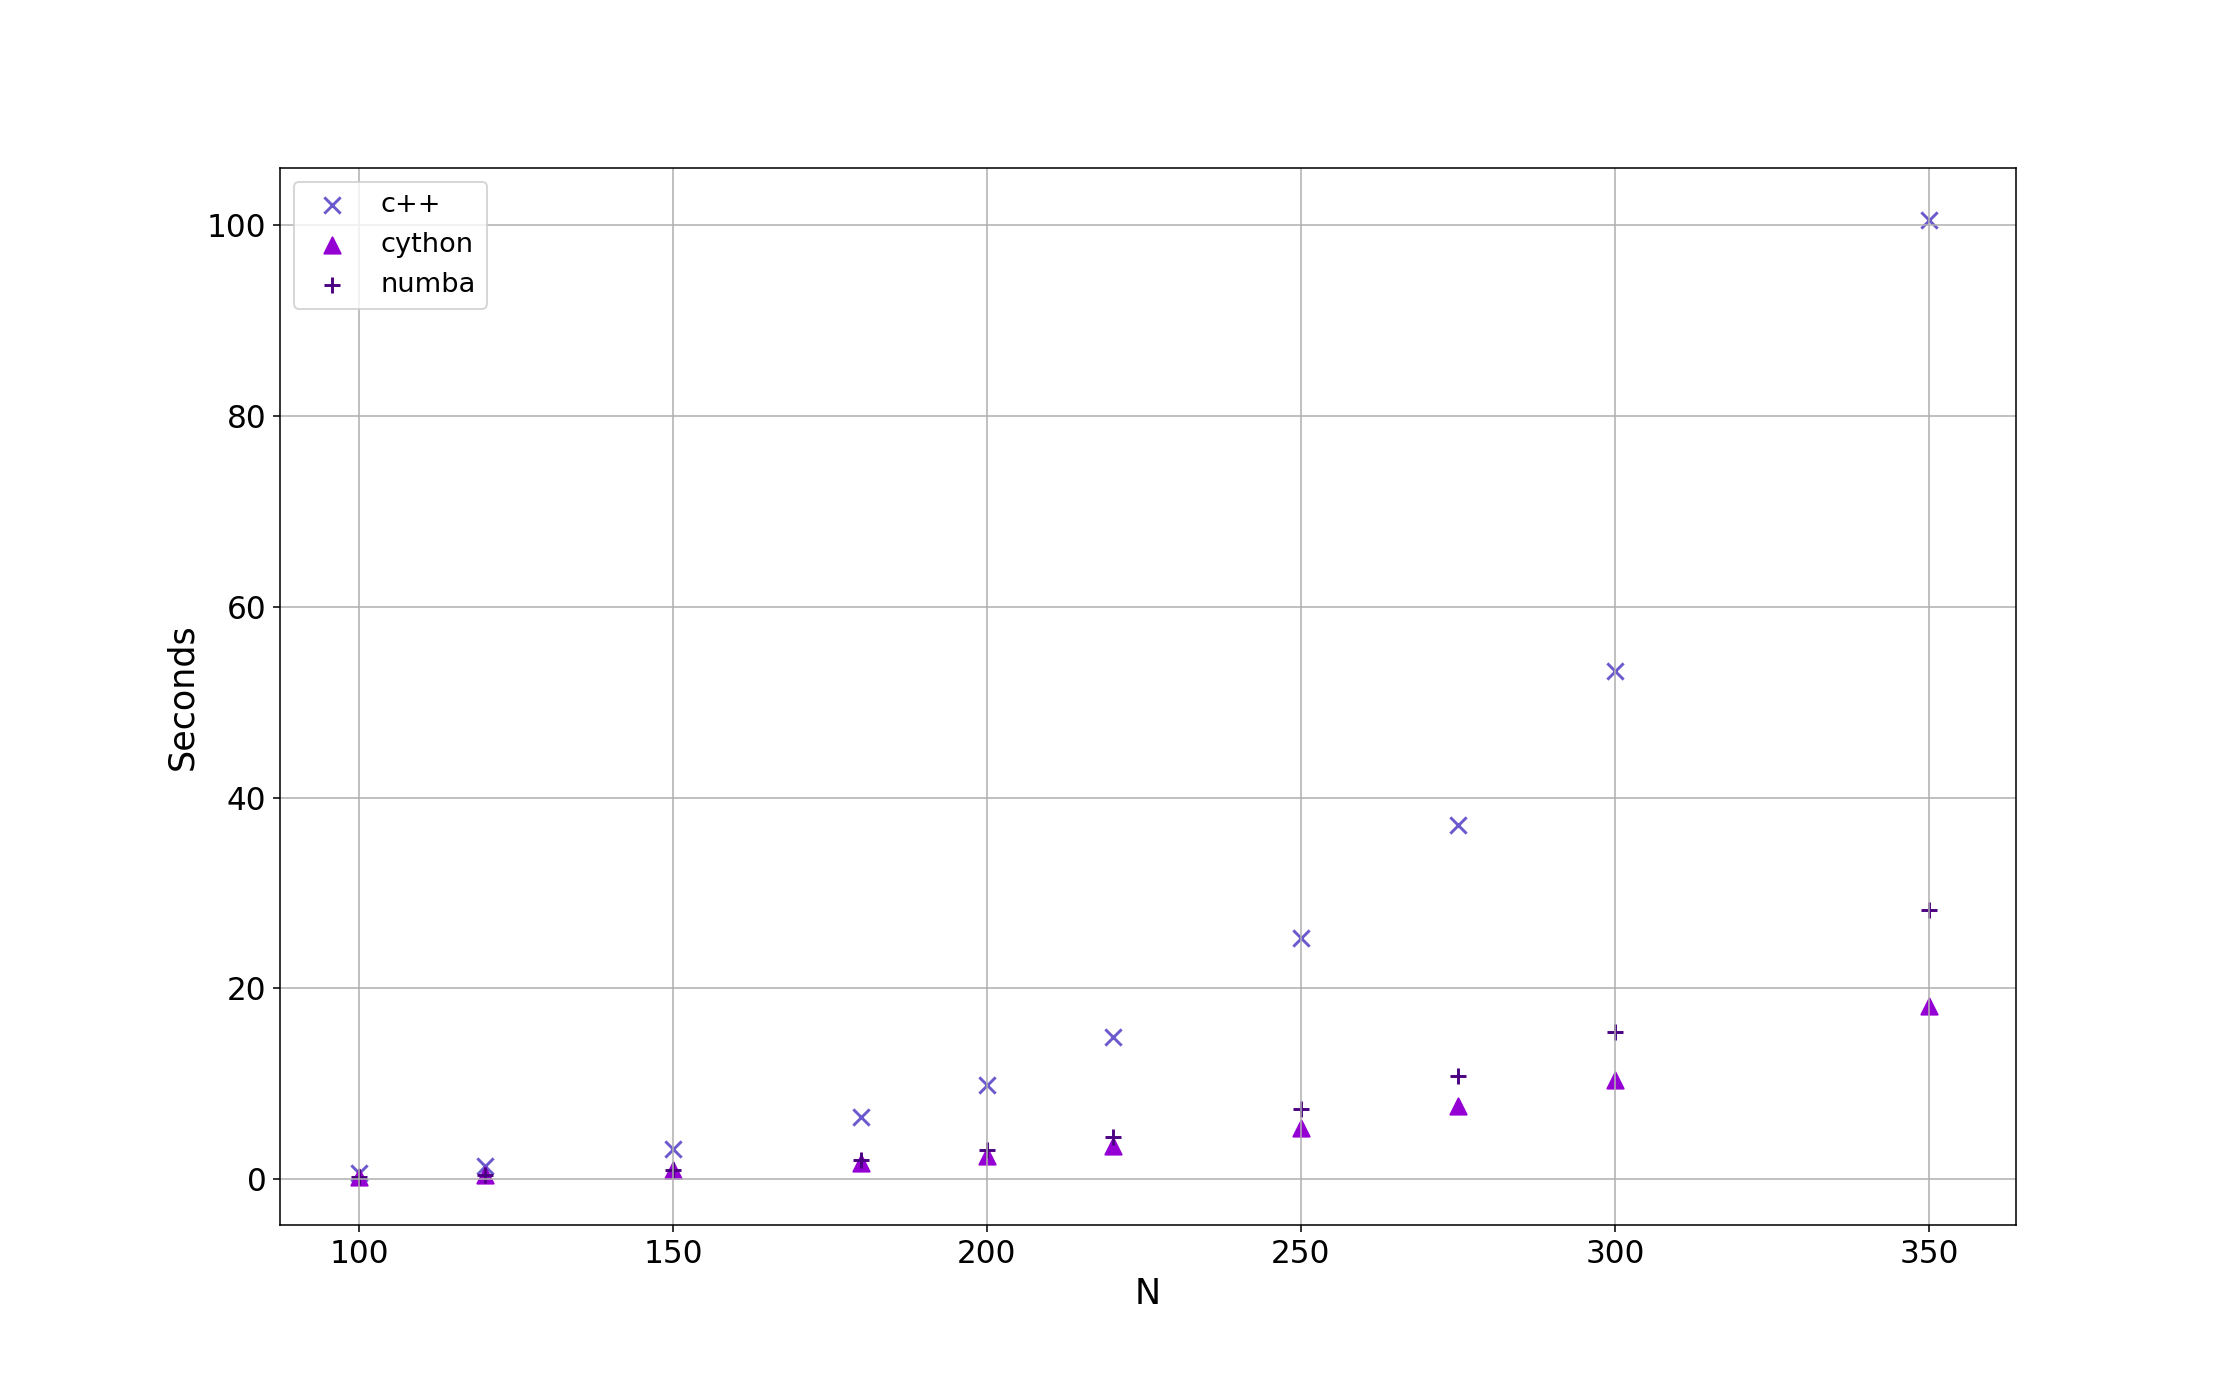
\includegraphics[width=1.0\textwidth]{../figures/speedComp_100_350.png}
  \caption{Average timing of 5 runs for the jacobi method implemented in c++, cython, numba. Starting from $N=100$ until $N=350$.}
  \label{fig:timing_largeN}
\end{figure}

\begin{figure}[H]
  \centering
  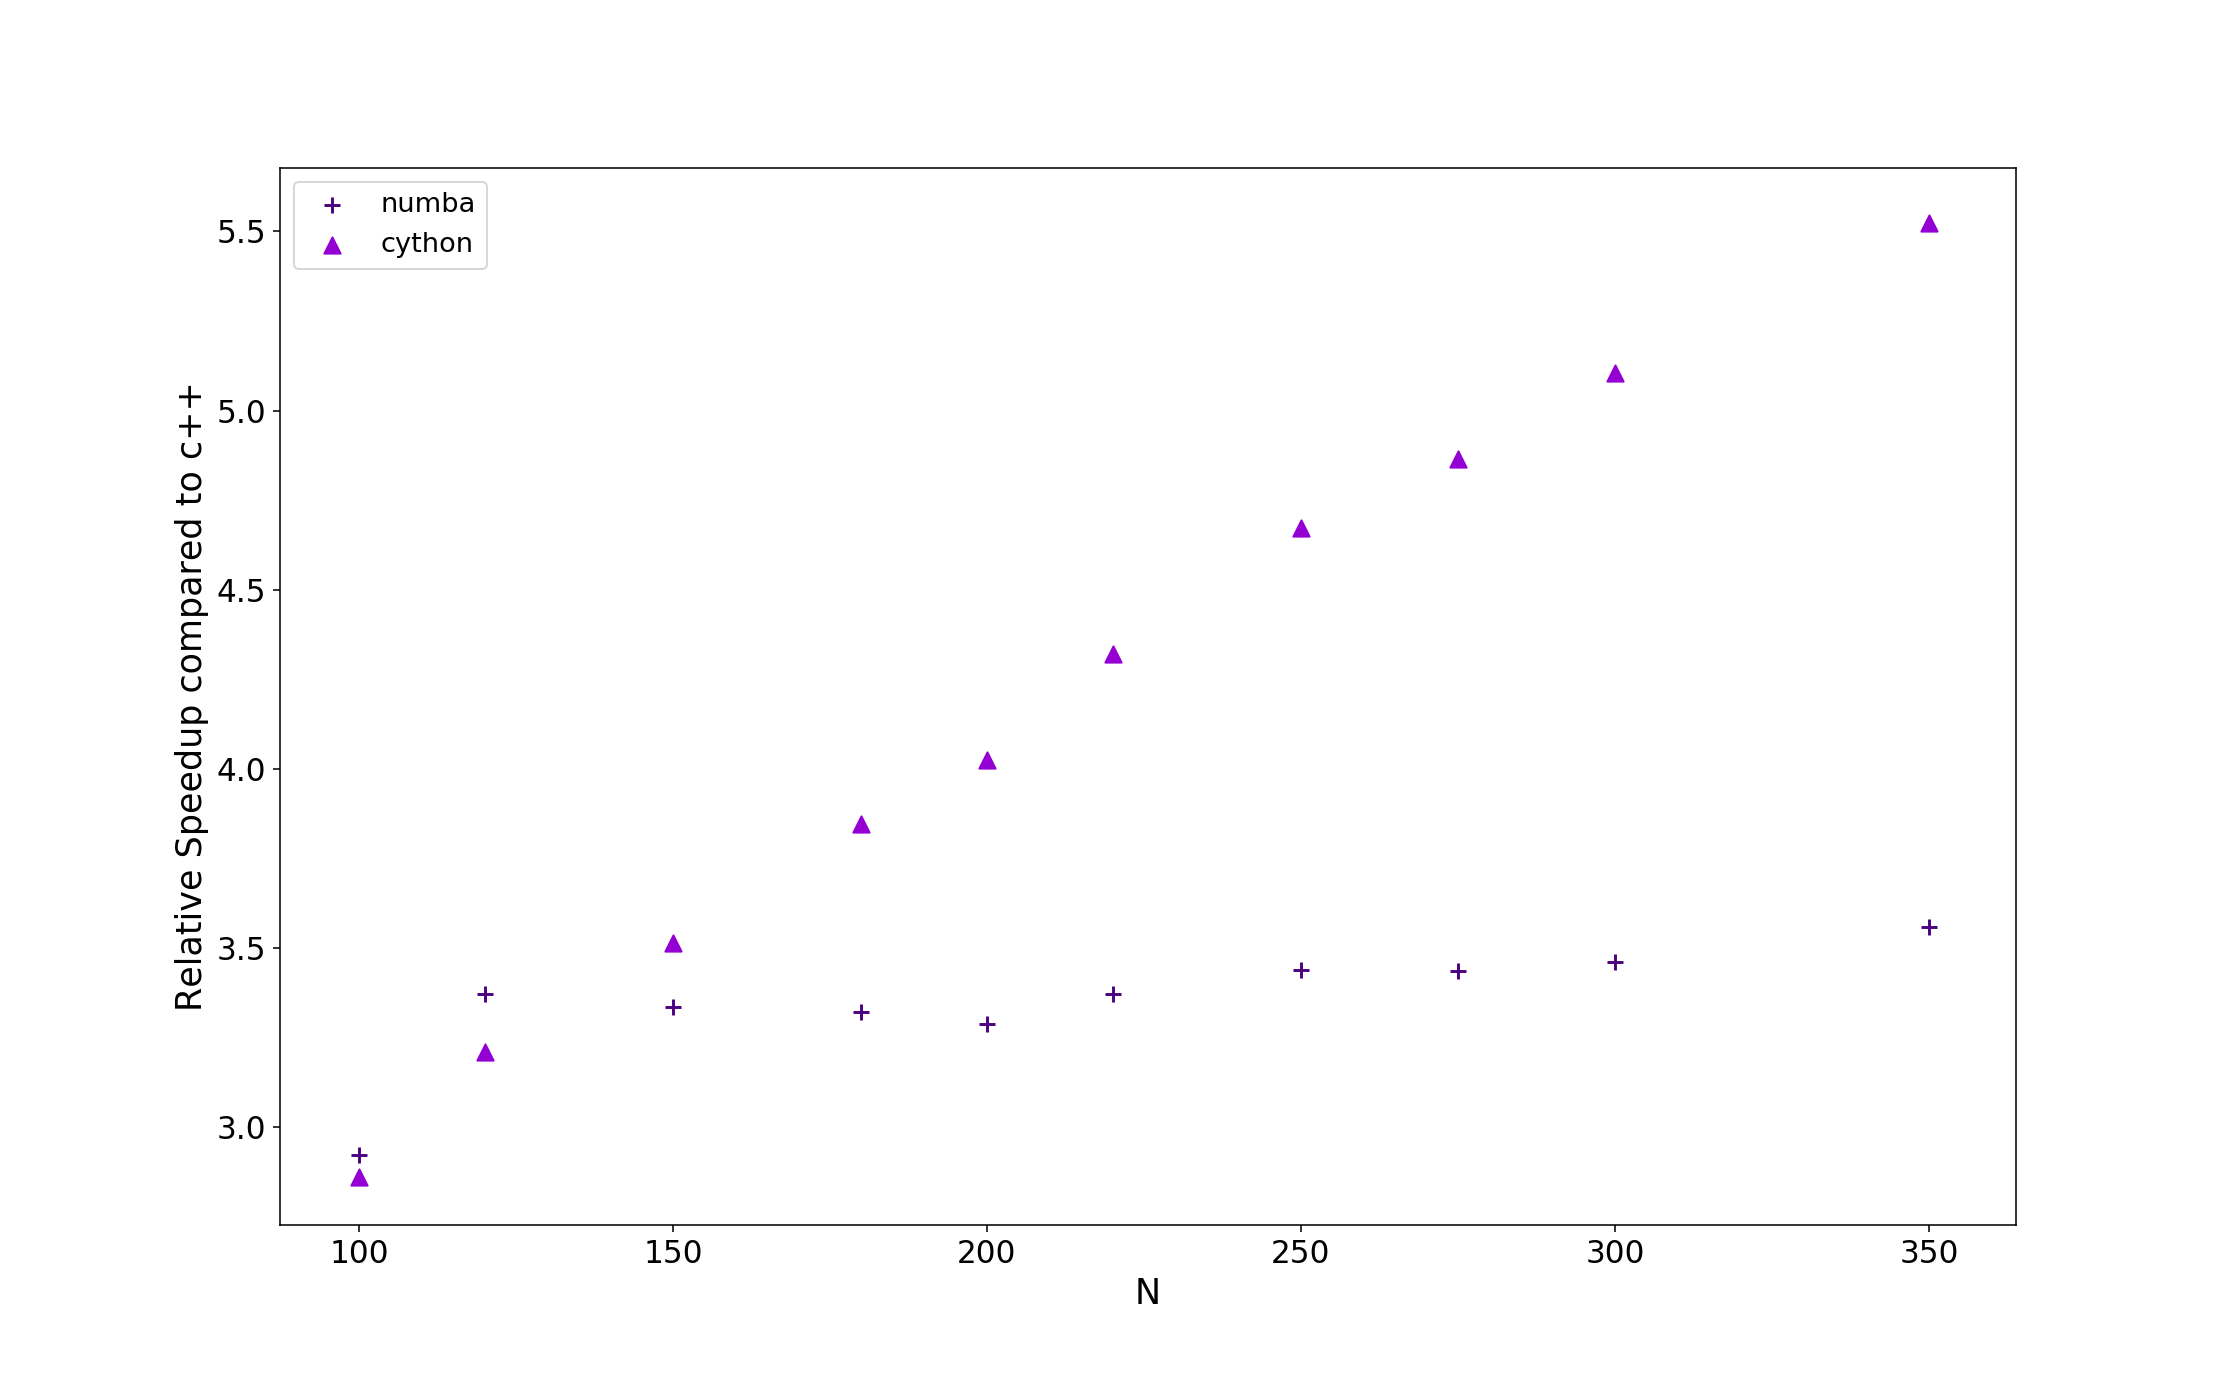
\includegraphics[width=1.0\textwidth]{../figures/speedCompC++_100_350.png}
  \caption{Relative speed up compared to c++}
  \label{fig:comp_c++}
\end{figure}

\subsection{Jacobi method c++ run time vs armadillo}
May not be relevant!

\begin{figure}[H]
  \centering
  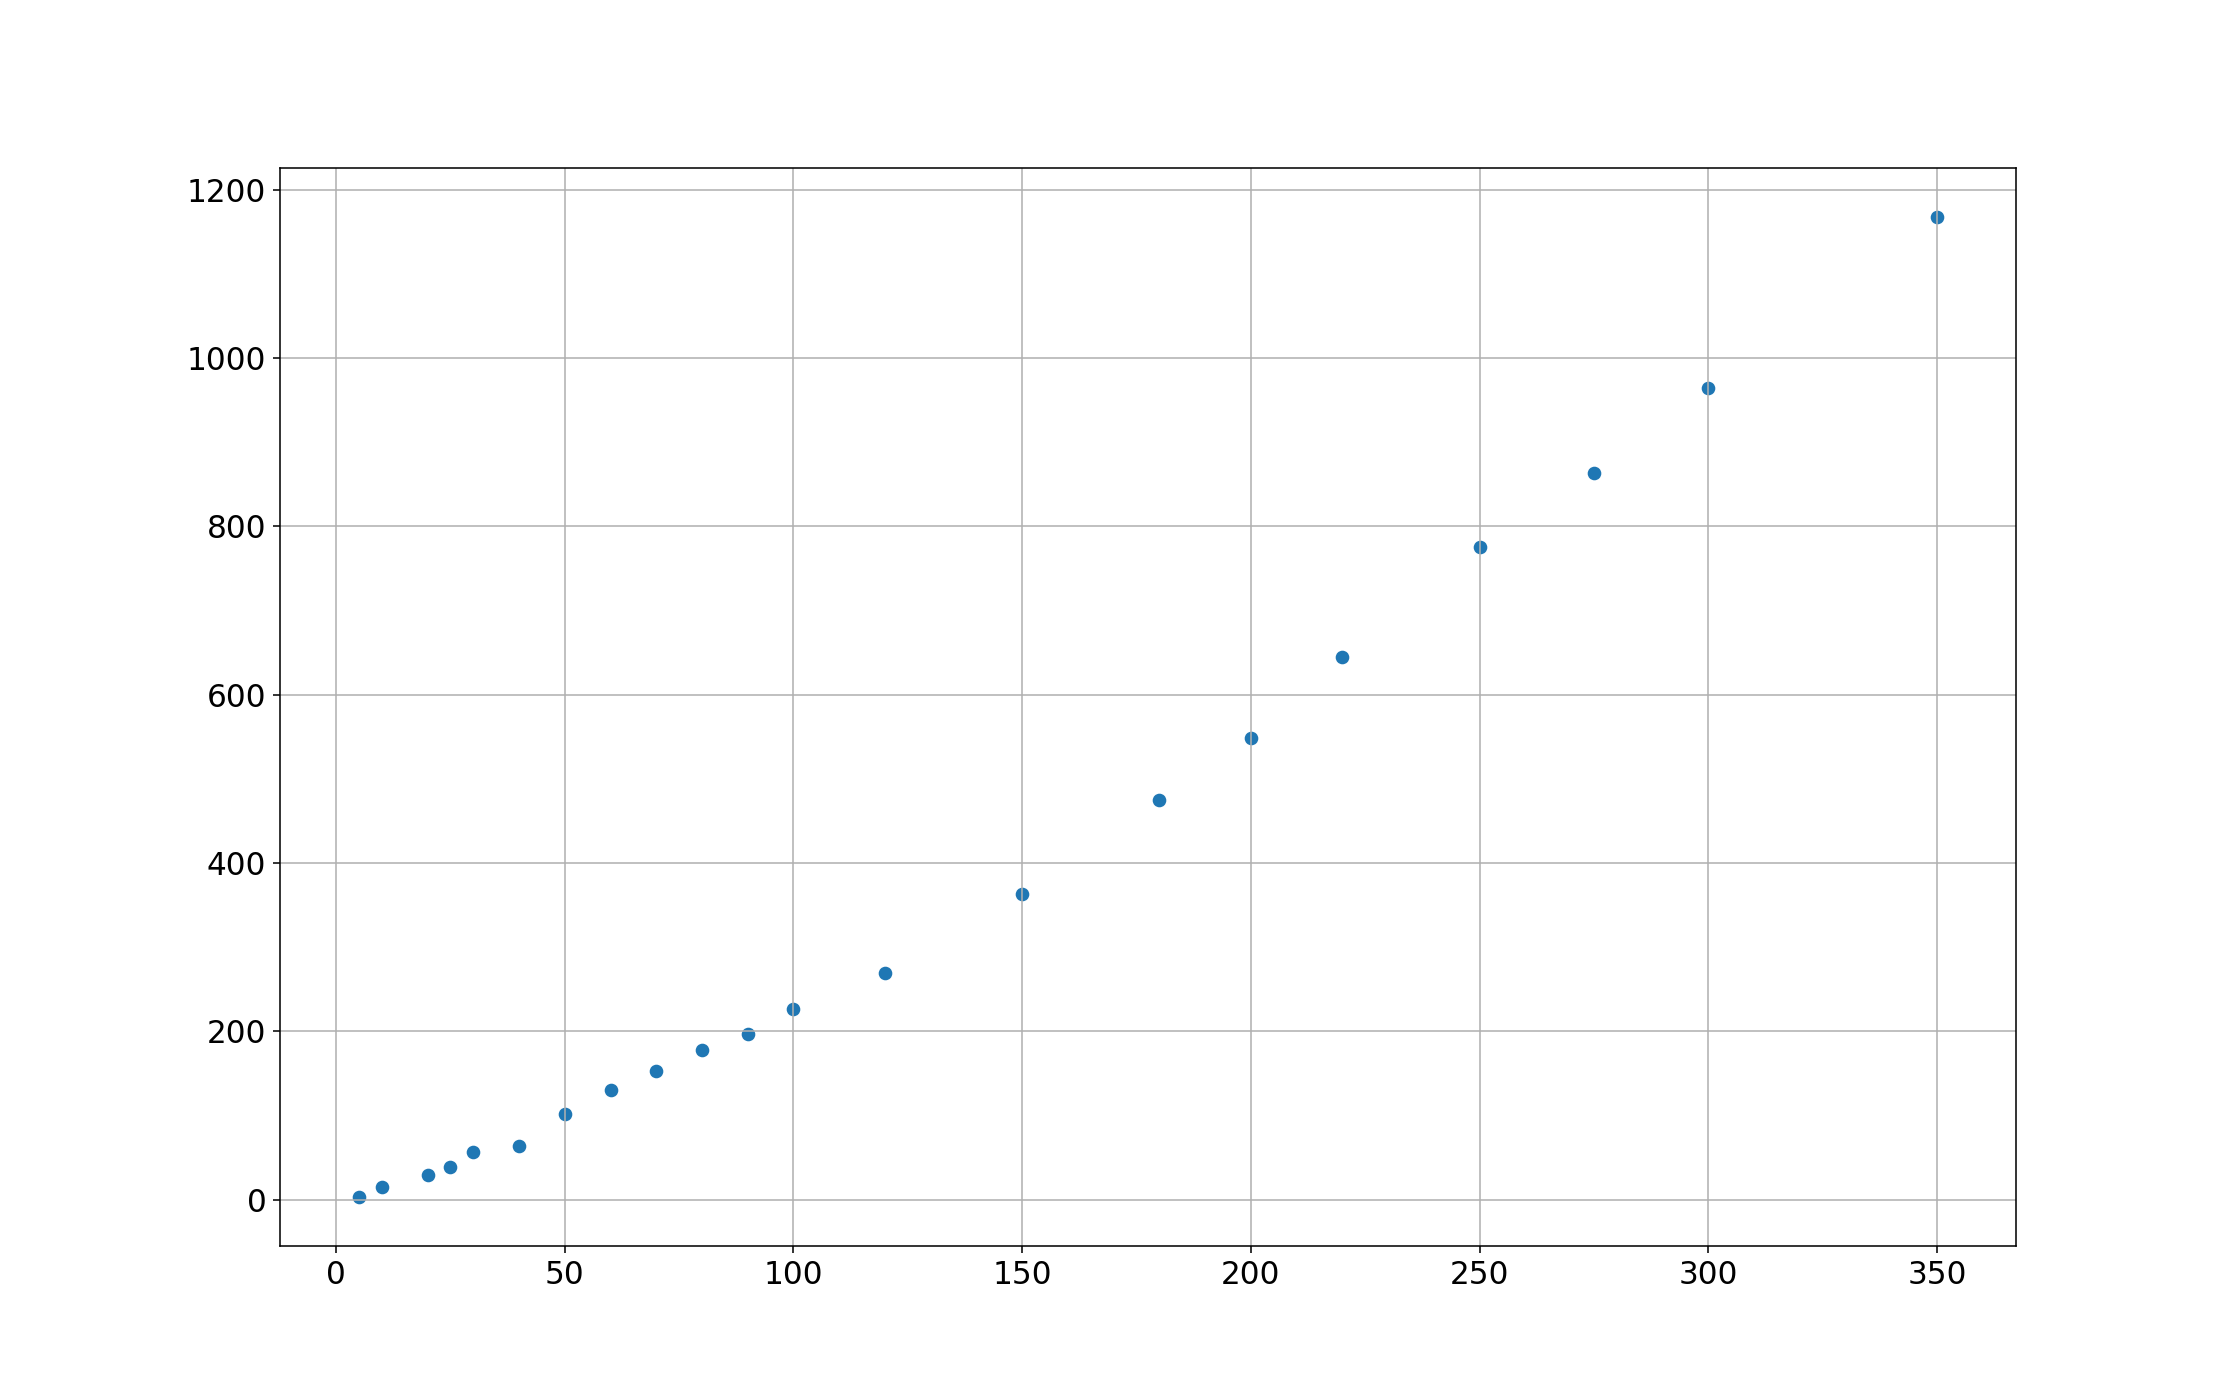
\includegraphics[width=0.66\textwidth]{../figures/compare_arma_cpp.png}

  \caption{Run time of the Jacobi method implemented in c++ divided by the run time of eigsys
  from armadillo. Average of three runs for all n.}

  \label{fig:cpp_arma}
\end{figure}




\subsection{Comparing run times of different implementations of the Jacobi method}
